%% =====================================================================
%% Same Abstract, Different Conclusion: A Controlled Study of Prompt
%% Sensitivity in LLM-Drawn Research Conclusions on PubMedQA
%%
%% Implementation paper (AI Tools for Research, Lab 02).
%% Compile: tectonic main.tex   (or pdflatex main && bibtex main && pdflatex main x2)
%% Every number below is produced by scripts/analyze.py -> results/tables/*.csv
%% =====================================================================
\documentclass[acmsmall,nonacm]{acmart}

\usepackage{booktabs}
\usepackage{tabularx}
\usepackage{array}
\usepackage{amsmath}
\usepackage{graphicx}
\usepackage{multirow}
\usepackage{tikz}
\usetikzlibrary{arrows.meta,positioning,fit}

\newcolumntype{L}[1]{>{\raggedright\arraybackslash}p{#1}}
\newcolumntype{Y}{>{\raggedright\arraybackslash}X}
\setcopyright{none}
\settopmatter{printacmref=false}
\renewcommand\footnotetextcopyrightpermission[1]{}

\title{Same Abstract, Different Conclusion: A Controlled Study of Prompt Sensitivity in LLM-Drawn Research Conclusions}

\author{Jagarlamudi Siva Sai Sumanth}
\affiliation{%
  \institution{Indian Institute of Information Technology Allahabad}
  \city{Prayagraj}
  \country{India}}
\renewcommand{\shortauthors}{J. S. S. Sumanth}

%% ABSTRACT -- written last, after all results were final.
\begin{abstract}
Researchers increasingly ask large language models (LLMs) to state what a study concludes, and they fix one prompt to do so. We test whether that conclusion survives equally reasonable rewordings of the prompt. On the official 500-abstract PubMedQA test set, two small open instruction-tuned models (Qwen2.5-0.5B and Llama-3.2-1B) were scored under 14 prompts in three families: paraphrase, surface format, and underspecification. A parse-free protocol reads the model's probabilities for yes/no/maybe directly. The setup was validated first: a majority-class baseline reproduces the published 55.2\% accuracy and 23.71 macro-F1 exactly. Rewording a fully specified prompt changed the conclusion for 63.4\% (Qwen) and 97.6\% (Llama) of abstracts. Prompts with near-identical accuracy reached opposite conclusions; for example, Llama said ``yes'' to 98\% of studies under one prompt and ``no'' to 66\% under another. Two analysts using different single prompts agreed on only 52--61\% of studies. Which kind of prompt change mattered most depended on the model, and every configuration with a low flip rate achieved it by giving nearly the same answer to every abstract. Reproducing contextual calibration did not improve macro-F1 for either model. It drove one model to answer almost always ``yes'' and the other almost always ``maybe'' (accuracy 11.4\%), because the empty-input answer the method treats as bias is a legitimate abstention in this task. Ensembling diverse prompts was the only intervention that improved both accuracy (Llama: 55.8\% to 60.4\%, McNemar $p=0.001$) and agreement between analysts (to 93\% with four prompts). Validation also showed that a repetition penalty in one model's shipped decoding defaults silently changed 6 of 40 greedy conclusions. We recommend reporting conclusion-level stability together with the diversity of predictions, and publishing decoding defaults, whenever LLMs are used to read research evidence.
\end{abstract}

\keywords{prompt sensitivity, reproducibility, contextual calibration, evidence synthesis, PubMedQA, small language models}

\begin{document}
\maketitle

%% =====================================================================
\section{Introduction}
\label{sec:intro}

Researchers increasingly ask large language models (LLMs) to read a study and state what it concludes, for example when they screen or code evidence in a systematic review. In such use, one prompt is written, fixed, and applied to every study. Our earlier literature review~\cite{sumanth2026review} argued that this practice hides a researcher degree of freedom~\cite{gelman2013forking}. Many equally reasonable prompts exist, and the literature shows that semantically equivalent prompts can move benchmark accuracy by tens of points~\cite{sclar2024formatting,mizrahi2024stateofwhatart,errica2025sensitivity}. The review's central open question (its Section~7.2) was whether this benchmark-level sensitivity also shows up at the level that matters for research: \emph{does the conclusion drawn from a single study change when the prompt is reworded?}

This paper tests that question experimentally. We use PubMedQA~\cite{jin2019pubmedqa}, in which each of 1{,}000 PubMed abstracts is paired with a research question and an expert yes/no/maybe conclusion. The abstract's own conclusion section is withheld from the model, so the task is a direct operationalisation of ``read the evidence and state the conclusion.'' We score two small, open, locally run instruction-tuned models on the official 500-item test set under 14 prompts. The prompts fall into three families that isolate mechanisms identified in the review: semantic paraphrase, surface formatting, and task underspecification. We then reproduce a published mitigation, contextual calibration~\cite{zhao2021calibrate}, and test multi-prompt ensembling.

We ask three research questions:
\begin{description}
  \item[RQ1] How often does the conclusion for the same abstract change across semantically equivalent prompts?
  \item[RQ2] Which kind of prompt change (paraphrase, format, underspecification) destabilises conclusions most, and how does prompt variation compare with run-to-run sampling variation?
  \item[RQ3] Do contextual calibration and ensembling make conclusions more stable \emph{and} more accurate than a single prompt?
\end{description}

\noindent\textbf{Contributions.} Prompt sensitivity on PubMedQA has already been measured~\cite{hariprasad2026clinical,sadanandan2026cot}, so we do not claim to be the first to measure it. Our contributions are the following:
(i)~a controlled, parse-free protocol that measures stability \emph{at the level of conclusions} (flip rate, Fleiss'~$\kappa$, and a ``two-analyst'' agreement metric), alongside accuracy;
(ii)~a family-level comparison of prompt changes under equal set sizes;
(iii)~a reproduction of contextual calibration, which shows when its stability gains are \emph{degenerate};
(iv)~a baseline-validation finding: a decoding default shipped with one model silently changes greedy conclusions.
All code, raw per-item probabilities, logs and figures are released for reproduction.

%% =====================================================================
\section{Related Work}
\label{sec:related}

\textbf{Prompt sensitivity.} Zhao et al.~\cite{zhao2021calibrate} traced few-shot instability to majority-label, recency and common-token biases. Lu et al.~\cite{lu2022fantastically} showed that example order alone moves accuracy from near chance to near state of the art. Sclar et al.~\cite{sclar2024formatting} found spreads of up to 76 accuracy points across meaning-preserving formats. Mizrahi et al.~\cite{mizrahi2024stateofwhatart} showed that model \emph{rankings} change across instruction paraphrases and argued for multi-prompt evaluation. Errica et al.~\cite{errica2025sensitivity} defined instance-level \emph{sensitivity} and \emph{consistency} metrics, which we adopt. Pecher et al.~\cite{pecher2026underspecification} attributed much of the observed sensitivity to underspecified prompts. Hua et al.~\cite{hua2025flaw} argued that part of it is an artifact of rigid answer parsing, which motivates our parse-free scoring. Cao et al.~\cite{cao2024worst} emphasised worst-prompt performance and found that existing consistency methods help little. Barrie et al.~\cite{barrie2024pss} adapted inter-coder reliability to text annotation as a ``prompt stability score''; our use of Fleiss'~$\kappa$ follows the same logic.

\textbf{Biomedical question answering.} PubMedQA~\cite{jin2019pubmedqa} reports a majority-class baseline of 55.2\% accuracy, a fine-tuned BioBERT result of 68.1\%, and single-human performance of 78.0\%. Two recent studies examine prompt sensitivity on it. Hariprasad~\cite{hariprasad2026clinical} evaluates five small open models under five prompt \emph{styles} and finds that consistency and accuracy are largely independent: models can be ``reliably wrong.'' Sadanandan and Behzadan~\cite{sadanandan2026cot} report that chain-of-thought and few-shot prompting reduce MedGemma accuracy and that shuffling answer options changes 59.1\% of predictions. We differ in three ways. We hold the instruction's meaning fixed within families of equal size. We score answer distributions rather than parsed text. And we test whether mitigations change \emph{conclusion-level} stability.

%% =====================================================================
\section{Method}
\label{sec:method}

\begin{figure}[t]
\centering
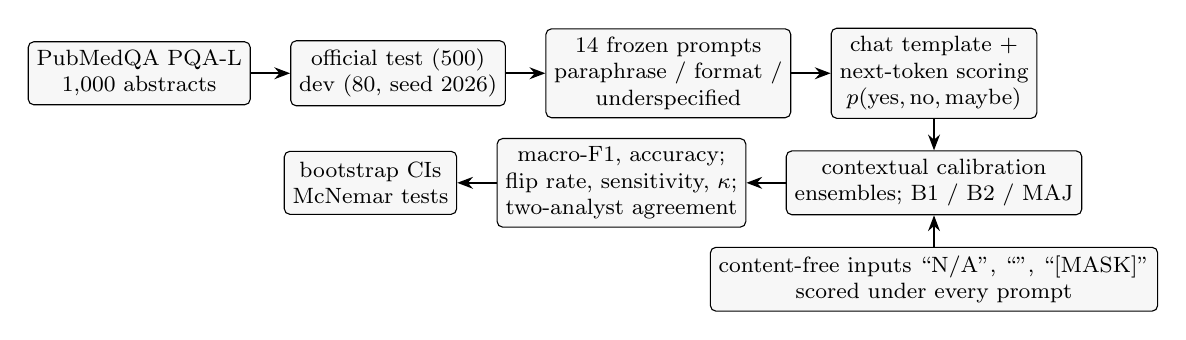
\begin{tikzpicture}[node distance=4mm and 5mm, every node/.style={font=\footnotesize, align=center},
  box/.style={draw, rounded corners=2pt, minimum height=8mm, inner sep=3pt, fill=gray!6},
  arr/.style={-{Stealth[length=2mm]}, thick}]
\node[box] (data) {PubMedQA PQA-L\\1{,}000 abstracts};
\node[box, right=of data] (split) {official test (500)\\dev (80, seed 2026)};
\node[box, right=of split] (prompt) {14 frozen prompts\\paraphrase / format /\\underspecified};
\node[box, right=of prompt] (score) {chat template +\\next-token scoring\\$p(\text{yes},\text{no},\text{maybe})$};
\node[box, below=of score] (mit) {contextual calibration\\ensembles; B1 / B2 / MAJ};
\node[box, left=of mit] (met) {macro-F1, accuracy;\\flip rate, sensitivity, $\kappa$;\\two-analyst agreement};
\node[box, left=of met] (stat) {bootstrap CIs\\McNemar tests};
\node[box, below=of mit] (cf) {content-free inputs ``N/A'', ``'', ``[MASK]''\\scored under every prompt};
\draw[arr] (data) -- (split); \draw[arr] (split) -- (prompt); \draw[arr] (prompt) -- (score);
\draw[arr] (score) -- (mit); \draw[arr] (mit) -- (met); \draw[arr] (met) -- (stat);
\draw[arr] (cf) -- (mit);
\end{tikzpicture}
\caption{Experimental pipeline. The protocol, prompts and seeds were frozen before any test-split prediction was produced.}
\Description{A flow diagram: dataset, split, prompts, scoring, then mitigations and baselines, metrics, and statistics. Content-free inputs also feed the scoring step.}
\label{fig:pipeline}
\end{figure}

\subsection{Task and data}
Each PubMedQA PQA-L item has a question (usually the article title phrased as a question), the abstract's sections without the conclusion, and an expert label in \{yes, no, maybe\}. We use the official 500-item test split (yes 276, no 169, maybe 55) and an 80-item dev split sampled with seed 2026 from the remaining items. The dev split is used only to select the B2 prompt and the majority class. A unit test checks that the conclusion text never appears in the model input, and the loader asserts that our test labels match the official ground-truth file. The data are MIT-licensed.

\subsection{Models}
We use Qwen2.5-0.5B-Instruct~\cite{qwen2025report} and Llama-3.2-1B-Instruct~\cite{grattafiori2024llama3}. Weight revisions are pinned by commit hash in the configuration. Both run in fp16 on an Apple M1 laptop with 8\,GB of memory, which is the setting of a researcher running models locally on sensitive material. A third model (Qwen2.5-1.5B-Instruct) was in the frozen plan but was dropped for time before any of its outputs existed; we return to this in Section~\ref{sec:limits}.

\subsection{Prompts}
Table~\ref{tab:prompts} summarises the 14 prompts; the full texts are in \texttt{src/prompts.py}. The canonical prompt P0 fully specifies the task. It names a systematic-review context, defines each label, and asks for one word. The \emph{paraphrase} family (P0--P4) rewords P0 and keeps its specification and layout. The \emph{format} family (P0, F1--F4) keeps P0's words and changes only separators, casing, field names or the order of fields. The \emph{underspecified} family (M1--M5) omits the label definitions and the output format. Each family has exactly five prompts, so stability metrics are comparable across families.

\begin{table}[t]
\caption{Prompt families. P0 belongs to both the paraphrase and format families.}
\label{tab:prompts}
\footnotesize
\begin{tabularx}{\linewidth}{@{}lL{0.17\linewidth}Y@{}}
\toprule
\textbf{ID} & \textbf{Family} & \textbf{What differs from P0} \\
\midrule
P0 & canonical & ``You are assisting with a systematic review\ldots Answer `yes' if the evidence supports a positive answer, `no' if \ldots negative, `maybe' if \ldots inconclusive or mixed. Respond with exactly one word\ldots'' \\
P1--P4 & paraphrase & Same specification, reworded (``evidence synthesis'', ``careful reviewer'', ``infer the study's conclusion'', \ldots) \\
F1--F4 & format & \texttt{\#\#\#} headers; ALL CAPS; question before abstract; \texttt{PASSAGE :::}\,/\,\texttt{QUERY :::} fields \\
M1--M5 & underspecified & Abstract and question only (in either order), ``Context:/Question:'', ``Read \ldots and answer'', ``What does this study conclude?'' \\
\bottomrule
\end{tabularx}
\end{table}

\subsection{Parse-free conclusion scoring}
Each rendered prompt is wrapped in the model's chat template. We then read the next-token distribution at the first assistant position. Let $T_\ell$ be the single-token surface forms of label $\ell$ (e.g.\ ``yes'', ``Yes'', ``YES''). We define
\begin{equation}
  p(\ell \mid x) = \frac{\sum_{t \in T_\ell} \pi(t \mid x)}{\sum_{\ell'} \sum_{t \in T_{\ell'}} \pi(t \mid x)}, \qquad \hat{y}(x) = \arg\max_\ell p(\ell \mid x),
\end{equation}
where $\pi$ is the model's softmax over the full vocabulary. The denominator, the \emph{label mass}, is logged as a measure of instruction following. Scoring avoids free-text parsing, a known source of inflated sensitivity~\cite{hua2025flaw}, and it is deterministic for a fixed model, dtype and device. Llama-3.2's chat template inserts the current date into its system header, so we pass a fixed date to keep prompts identical across days.

\subsection{Comparators and mitigations}
We compare the following:
\begin{itemize}
  \item \textbf{MAJ}, which predicts the dev majority class (``yes'');
  \item \textbf{B1}, the single canonical prompt P0, which is what a typical study does;
  \item \textbf{B2}, the single prompt with the best dev macro-F1, i.e.\ ``prompt engineering'';
  \item \textbf{CC}, contextual calibration of P0~\cite{zhao2021calibrate}: $q \propto p \oslash \hat{p}_{\text{cf}}$, where $\hat{p}_{\text{cf}}$ is the label distribution averaged over the content-free inputs ``N/A'', ``'' and ``[MASK]'' placed in the same prompt;
  \item \textbf{ENS}, the average of label distributions over the paraphrase family (5 prompts) or over all 14;
  \item \textbf{ENS+CC}, the same ensembles applied to calibrated distributions.
\end{itemize}

\subsection{Metrics}
The primary accuracy metric is macro-F1, because ``maybe'' is rare (11\%). For a set of $K$ prompts with predictions $\hat{y}_k(x)$ we compute:
\begin{itemize}
  \item instance \emph{sensitivity}~\cite{errica2025sensitivity}, $S(x) = \binom{K}{2}^{-1} \sum_{i<j} \mathbb{1}[\hat{y}_i(x) \neq \hat{y}_j(x)]$, averaged over abstracts;
  \item the \emph{flip rate}, the share of abstracts whose conclusion is not identical under all $K$ prompts;
  \item Fleiss'~$\kappa$, treating prompts as raters;
  \item the range of accuracy and macro-F1 across prompts.
\end{itemize}
Stability can be achieved trivially by always giving the same answer, so every stability figure is reported together with the share of predictions in the most common label. To estimate the practical risk we define \emph{two-analyst agreement}. Two analysts each draw $k$ distinct prompts from the nine fully specified prompts (paraphrase plus format) and report the ensemble conclusion; the metric is the share of abstracts on which they agree. We average it over 500 random draws. To compare prompt variation with run-to-run variation, we draw 10 samples per prompt from the temperature-scaled label distribution ($T \in \{0.7, 1.0\}$) and compute within-prompt pairwise disagreement.

\subsection{Statistics and protocol}
Confidence intervals are 95\% percentile bootstraps over abstracts (2{,}000 resamples, seed 2026). Accuracy differences against B1 use exact McNemar tests. The prompts, splits, metrics, seeds and decision rules (a flip rate of at least 10\% counts as ``unstable''; a mitigation ``helps'' if it improves macro-F1, or lowers the flip rate without lowering macro-F1) were frozen in \texttt{configs/experiment.json} before test predictions were generated. Protocol changes made after freezing (speed and loading fixes that did not change the results) are logged in the repository. Scoring 2 models $\times$ 14 prompts $\times$ 580 items (16{,}240 forward passes) took 3.7\,h on the M1 GPU (0.52\,s and 0.95\,s per pass).

%% =====================================================================
\section{Results}
\label{sec:results}

\subsection{Baseline validation}
\label{subsec:validation}
The checks below were run before any comparison (details in \texttt{baseline\_validation.md}).
\begin{itemize}
  \item \textbf{Published baseline reproduced.} The majority-class baseline gives 55.20\% accuracy and 23.71 macro-F1 on the test split, matching Table~5 of Jin et al.~\cite{jin2019pubmedqa} exactly.
  \item \textbf{Scorer is deterministic.} Re-scoring 20 dev items gave the same predictions, with probabilities within 0.01 (fp16 noise). Batched and single-item scoring differ by at most 0.007.
  \item \textbf{Scorer agrees with generation.} For Llama, the scored answer matched the first word of greedy generation on 40/40 dev items. For Qwen it matched 35/40 at first. Diagnosis traced the gap to Qwen2.5's shipped \texttt{generation\_config}, which sets \texttt{repetition\_penalty=1.1}; transformers applies this even in greedy decoding. The penalty lowers ``maybe'', which occurs in the prompt, but not ``Yes'', which does not, and it changed the generated conclusion for 6 of 40 abstracts. With the penalty set to 1.0, agreement rose to 39/40, and the remaining case is a near-tie. Our scorer reads raw logits and is unaffected, but the episode shows that ``greedy'' chat output can depend on a decoding default that few researchers would report.
  \item \textbf{Both models are weak in absolute terms.} Each answered only 1 of 4 constructed sanity questions correctly. Under B1, Llama predicts ``yes'' for 98.2\% of abstracts and is statistically indistinguishable from MAJ (McNemar $p=0.45$). Qwen over-predicts ``maybe'' (45.8\%) and scores 35.8\% accuracy.
\end{itemize}
The stability findings below should be read as properties of small models.

\begin{table}[t]
\caption{Baselines and mitigations on the PubMedQA test set ($n=500$). Accuracy and macro-F1 in \%, with 95\% bootstrap CIs. ``Passes'' is forward passes per abstract; ``Maybe'' is the share of ``maybe'' predictions; $p$ is an exact McNemar test of accuracy against B1. B2 shows the prompt selected on dev.}
\label{tab:methods}
\footnotesize
\begin{tabular}{@{}llrllrl@{}}
\toprule
Model & Method & Passes & Accuracy & Macro-F1 & Maybe & $p$ vs B1 \\
\midrule
\csname @@input\endcsname tables/methods_test.tex
\bottomrule
\end{tabular}
\end{table}

\subsection{RQ1: Conclusions change for most abstracts}
\label{subsec:rq1}
Under the five fully specified paraphrases, the conclusion changed under at least one prompt for 63.4\% [59.2, 67.6] of abstracts with Qwen and 97.6\% [96.2, 99.0] with Llama (Table~\ref{tab:stability}). Both values are far above the pre-specified 10\% threshold (frozen before test predictions existed), so H1 is supported. For 308 of the 500 abstracts (61.6\%), the conclusion flips for \emph{both} models. Agreement across paraphrases is at chance level (Fleiss'~$\kappa$ = 0.11 and $-0.10$).

\emph{Accuracy hides this instability.} Llama's accuracy under P0--P3 lies in a narrow 53.8--56.4\% band, yet P0 concludes ``yes'' for 98.2\% of studies while P2 concludes ``no'' for 65.8\% (Figure~\ref{fig:shares}). Two prompts that would be reported as performing equally well reach opposite conclusions for most of the evidence base. This is Errica et al.'s~\cite{errica2025sensitivity} observation (aggregate accuracy conceals instance-level sensitivity) translated to the level of research conclusions. Figure~\ref{fig:perprompt} shows per-prompt macro-F1. Across all 14 prompts, macro-F1 spans 33.6 points for Qwen and 21.2 points for Llama.

\begin{figure}[t]
  \centering
  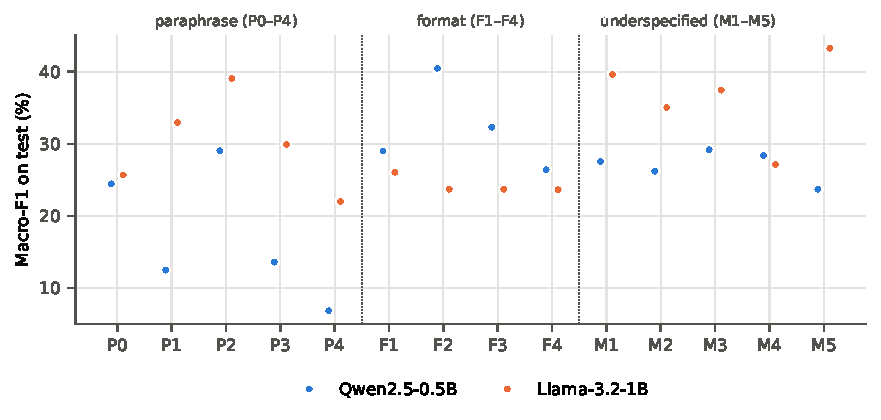
\includegraphics[width=\linewidth]{figures/fig_per_prompt_f1.pdf}
  \caption{Macro-F1 on the test set for each of the 14 prompts. Dotted lines separate the prompt families.}
  \Description{Dot plot with prompts on the x-axis and macro-F1 on the y-axis for two models. Qwen ranges from about 7 to 40; Llama from about 22 to 43. Which model scores higher changes from prompt to prompt.}
  \label{fig:perprompt}
\end{figure}

\begin{figure}[t]
  \centering
  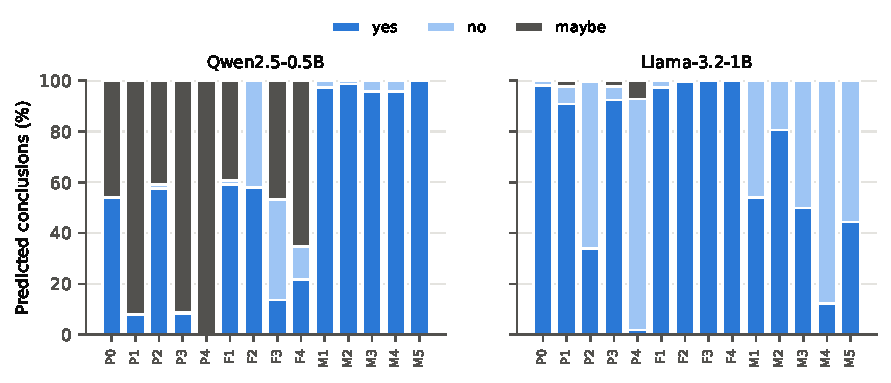
\includegraphics[width=\linewidth]{figures/fig_label_shares.pdf}
  \caption{Share of yes/no/maybe conclusions under each prompt. Each prompt mostly moves the model's default answer rather than its reading of individual abstracts.}
  \Description{Stacked bars per prompt for two models. Qwen is mostly maybe under P1, P3 and P4 and mostly yes under the underspecified prompts. Llama is mostly yes except under P2 and P4, where it is mostly no, and it is mixed under the underspecified prompts.}
  \label{fig:shares}
\end{figure}

\begin{table}[t]
\caption{Conclusion stability by prompt family (raw probabilities unless marked CC). Sens.\ = mean pairwise disagreement (Errica et al.); Flip = abstracts whose conclusion is not identical across the family (\%, 95\% CI); $\kappa$ = Fleiss' kappa; Acc.\ = range of accuracy across prompts; $\Delta$F1 = range of macro-F1. The last two columns repeat Flip and $\kappa$ after contextual calibration.}
\label{tab:stability}
\footnotesize
\begin{tabular}{@{}llrrlrlrrr@{}}
\toprule
Model & Family & $K$ & Sens. & Flip & $\kappa$ & Acc. & $\Delta$F1 & Flip$_{\text{CC}}$ & $\kappa_{\text{CC}}$ \\
\midrule
\csname @@input\endcsname tables/stability_test.tex
\bottomrule
\end{tabular}
\end{table}

\subsection{RQ2: The source of instability depends on the model}
\label{subsec:rq2}
Within each model the families differ clearly (non-overlapping CIs), but the ordering is reversed between the two models (Figure~\ref{fig:flips}). For Qwen, surface format is the most destabilising change (flip rate 94.6\%), ahead of paraphrase (63.4\%) and underspecification (7.2\%). For Llama, paraphrase (97.6\%) and underspecification (81.0\%) dominate, and format barely matters (3.0\%).

Every low flip rate coincides with a \emph{collapse} onto one label. Qwen predicts ``yes'' for 97.4\% of abstracts under the underspecified prompts, and Llama predicts ``yes'' for 99.0\% under the format prompts. Low instability is therefore not evidence of reliable reading. H2, which expected underspecified prompts to be the \emph{least} stable~\cite{pecher2026underspecification}, is contradicted for both models. For Llama the underspecified prompts were even the most accurate (M5: macro-F1 43.3, the best single Llama prompt). One caveat applies: under these prompts the probability mass on label tokens is low (0.00--0.38), meaning the model would not naturally answer with a bare label, so restricted scoring forces a choice.

\textbf{Prompt variance versus sampling variance.} Disagreement between paraphrases under greedy scoring (Qwen 34.6\%, Llama 52.9\%) is of the same size as within-prompt disagreement from sampling at $T=0.7$ (31.6\%, 46.0\%) or $T=1.0$ (41.7\%, 53.8\%). The two sources add: sampling across paraphrases at $T=1.0$ gives 49.8\% and 61.2\% (Figure~\ref{fig:variance}). The difference is that prompt effects are systematic. Repeating a run with the same prompt does not average them away, and a single published prompt fixes them for every study it is applied to.

\textbf{Model rankings.} Llama has the higher macro-F1 under 9 prompts and Qwen under 5. For 49.5\% of prompt pairs the two prompts disagree about which model is better, reproducing the ranking instability of Mizrahi et al.~\cite{mizrahi2024stateofwhatart} on a two-model, research-conclusion task.

\begin{figure}[t]
  \centering
  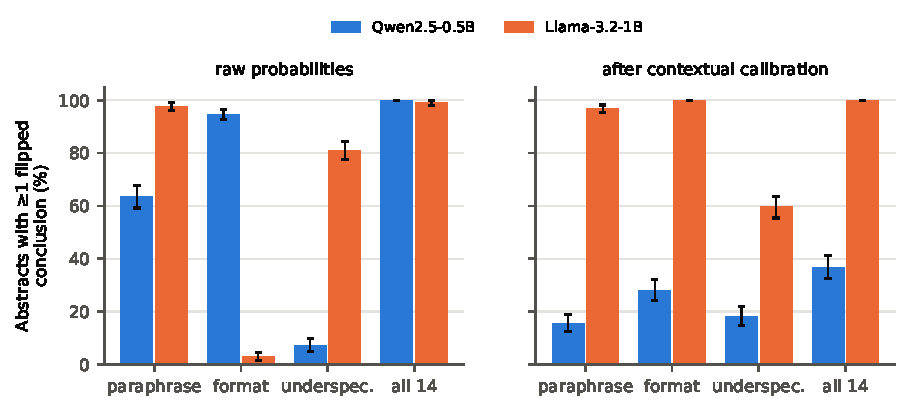
\includegraphics[width=\linewidth]{figures/fig_flip_rate_by_family.pdf}
  \caption{Share of abstracts whose conclusion changes within each prompt family (95\% bootstrap CIs), before and after contextual calibration.}
  \Description{Grouped bars. Raw: Qwen is highest for format (95\%) and lowest for underspecified (7\%); Llama is highest for paraphrase (98\%) and lowest for format (3\%). After calibration Qwen falls to 16--37\%, while Llama stays near 60--100\%.}
  \label{fig:flips}
\end{figure}

\begin{figure}[t]
  \centering
  \begin{minipage}[t]{0.49\linewidth}
    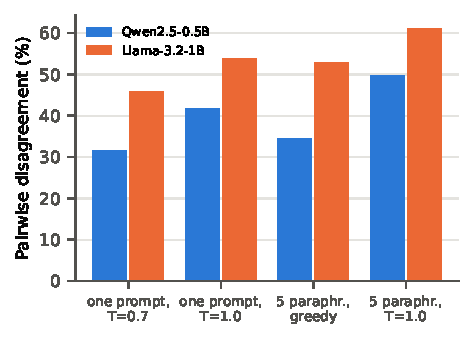
\includegraphics[width=\linewidth]{figures/fig_variance_sources.pdf}
    \caption{Pairwise disagreement from repeated sampling of one prompt versus across five paraphrases.}
    \Description{Bars comparing within-prompt sampling at T 0.7 and 1.0 with between-paraphrase disagreement. Between-paraphrase disagreement is similar to sampling at T 0.7 to 1.0, and highest when both are combined.}
    \label{fig:variance}
  \end{minipage}\hfill
  \begin{minipage}[t]{0.49\linewidth}
    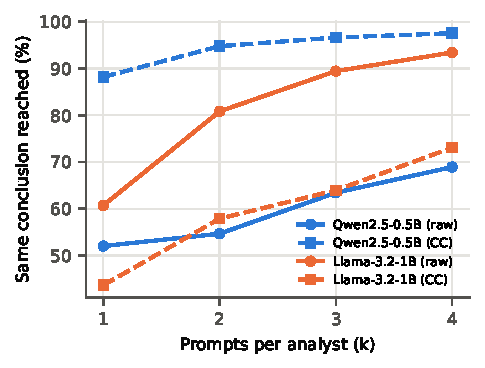
\includegraphics[width=\linewidth]{figures/fig_two_analyst_agreement.pdf}
    \caption{Probability that two analysts, each using $k$ different fully specified prompts, reach the same conclusion.}
    \Description{Lines for agreement against k from 1 to 4. Raw Llama rises from 61\% to 93\%; raw Qwen from 52\% to 69\%. Calibrated Qwen stays high (88--98\%); calibrated Llama is lowest (44--73\%).}
    \label{fig:twoanalyst}
  \end{minipage}
\end{figure}

\subsection{RQ3: Calibration fails; ensembling helps when prompt biases differ}
\label{subsec:rq3}
\textbf{Contextual calibration} did not improve macro-F1 for either model (Table~\ref{tab:methods}), so H3 is not supported. For Qwen, calibrated P0 scores 24.6 macro-F1 (vs 24.5 for B1) and predicts ``yes'' for 98.4\% of abstracts, which makes its accuracy identical to MAJ. For Llama, calibration is harmful: accuracy falls from 55.8\% to 11.4\% ($p<0.001$) as 99.6\% of predictions become ``maybe''. Calibration lowers Qwen's paraphrase flip rate from 63.4\% to 15.6\%, but only through the collapse onto ``yes''. Llama's flip rate is unchanged (96.8\%), and its two-analyst agreement drops (Figure~\ref{fig:twoanalyst}).

The content-free distributions explain both failures. For P0, Qwen answers the empty input with (yes, no, maybe) = (0.05, 0.40, 0.55) and Llama with (0.27, 0.73, 0.003). The calibration weights $1/\hat{p}_{\text{cf}}$ are therefore about 20 for Qwen's ``yes'' and about 330 for Llama's ``maybe''. Contextual calibration assumes that the answer to an empty input is pure bias~\cite{zhao2021calibrate}. Our conclusion task, however, contains an evidence-insufficient label, so ``maybe'' or ``no'' is arguably the \emph{correct} answer to ``N/A''. Calibration then penalises correct behaviour and inflates whichever label the model rightly avoided. We read this as a boundary condition of the method (instruction-tuned models; a task with an abstention-like class), not as a refutation of the original results.

\textbf{Ensembling} helps Llama. Averaging the five paraphrases raises macro-F1 from 25.7 to 37.3 and accuracy from 55.8\% to 59.8\% ($p=0.027$); averaging all 14 prompts gives 60.4\% ($p=0.001$). With a Bonferroni correction over the seven comparisons per model ($\alpha=0.007$), the 14-prompt gain remains significant, but the paraphrase-ensemble gain ($p=0.027$) does not. Two-analyst agreement rises from 60.7\% with one prompt to 89.4\% with three and 93.4\% with four. For Qwen, the paraphrase ensemble \emph{hurts} (macro-F1 16.8): the paraphrases share a ``maybe'' bias, and averaging reinforces it. The 14-prompt ensemble, which mixes prompts with opposite biases, helps (macro-F1 29.4). Ensembling therefore stabilises conclusions only when the prompt biases are diverse.

\textbf{Prompt selection on dev} (B2) gives the best macro-F1 for both models (Qwen 40.5 with F2; Llama 39.1 with P2), but the selected prompt does not transfer between models: F2 scores 23.7 on Llama, and P2 scores 29.0 on Qwen. For Llama, B2's accuracy is no different from B1's ($p=0.59$).

\subsection{Failure and error analysis}
\label{subsec:errors}
\begin{itemize}
  \item \textbf{The canonical prompt rarely concludes ``no''.} Under P0, recall of ``no'' studies is 1.2\% (Qwen) and 3.0\% (Llama), and Llama never concludes ``maybe''. A review that relied on this prompt would systematically over-report positive findings.
  \item \textbf{Confidence does not signal stability.} For Qwen, abstracts in the highest quartile of P0 confidence flip \emph{most} often across paraphrases (82.4\%, against 50.4--64.8\% in the other quartiles). For Llama the top quartile still flips 93.6\% of the time.
  \item \textbf{A concrete case.} For ``Is halofantrine ototoxic?'' (gold: yes; the authors conclude that it ``can be considered an ototoxic drug''), Llama answers yes under P0, P3 and F1--F4, maybe under P1 and P4, and no under P2. The same evidence yields all three conclusions depending only on the wording.
\end{itemize}

%% =====================================================================
\section{Discussion}
\label{sec:discussion}
For the small models studied here, the conclusion an LLM draws from a study abstract depends on the prompt for most abstracts. The dependence is largely invisible in the aggregate accuracy that is usually reported. Three implications for LLM-assisted evidence synthesis follow; all are conditional on the model scale we could test.

\emph{First, report conclusion-level stability, not only accuracy.} Prompts with the same accuracy reached opposite conclusions. Flip rate or two-analyst agreement, reported next to the modal-label share, exposes this; accuracy does not.

\emph{Second, low instability can be degenerate.} Every ``stable'' configuration in our data, including the calibrated Qwen model, achieved its stability by giving almost the same answer to every abstract. Stability metrics need a companion check on the diversity of predictions, a point that complements Hariprasad's observation that models can be ``reliably wrong''~\cite{hariprasad2026clinical}.

\emph{Third, mitigations must match the task.} Contextual calibration, one of the mitigations our review highlighted, failed in two different directions because the task has a legitimate answer for empty input. Multi-prompt ensembling was the only intervention that improved both accuracy and agreement, and only when the pooled prompts carried diverse biases. This qualifies the review's recommendation of multi-prompt evaluation~\cite{mizrahi2024stateofwhatart}: the \emph{choice} of prompt pool matters.

Our results are consistent with the concern of Hua et al.~\cite{hua2025flaw} that evaluation artifacts inflate sensitivity, but they also show its limits. Even with parsing removed entirely, conclusions flipped for 63--98\% of abstracts. The validation finding about Qwen's shipped repetition penalty shows that harness defaults are a further, separate source of variation that researchers seldom report.

%% =====================================================================
\section{Limitations and Threats to Validity}
\label{sec:limits}
\begin{itemize}
  \item \textbf{Scale.} Only two small models (0.5B and 1B) were tested, and both perform close to the majority class. The frozen plan included Qwen2.5-1.5B, but it was dropped for time before any of its outputs existed. Larger models may be more stable, so our effect sizes should not be generalised to frontier systems.
  \item \textbf{Task.} One dataset and a three-way label. PubMedQA questions are derived from article titles.
  \item \textbf{Prompts.} The 14 prompts were written by one author, so the space of equivalent prompts is only partly sampled.
  \item \textbf{Scoring.} Restricted scoring removes parsing artifacts but differs from free-text chat use. It forces a label even when label mass is low, notably for the underspecified prompts.
  \item \textbf{Sampling analysis.} Sampling variance was simulated from the restricted label distribution rather than from full decoding.
  \item \textbf{Calibration inputs.} Contextual calibration used the three content-free inputs of the original paper; other inputs, or label subsets, might behave differently.
  \item \textbf{Protocol.} The decision rules were written after dev-set (not test-set) accuracies for one model had been printed. The single-run fp16 MPS numerics can flip near-ties (maximum probability difference observed: 0.01).
\end{itemize}

%% =====================================================================
\section{Conclusion}
\label{sec:conclusion}
We asked whether prompt sensitivity, well documented at the benchmark level, also destabilises the conclusions an LLM draws from individual research abstracts. On PubMedQA, with two small open models and a parse-free protocol, it does. Rewording a fully specified prompt changed the conclusion for 63--98\% of abstracts. Prompts with equal accuracy reached opposite conclusions, and two analysts using different single prompts agreed on only 52--61\% of studies. A reproduced mitigation, contextual calibration, failed in this setting because the empty-input answer it treats as bias is a legitimate abstention. Multi-prompt ensembling with diverse prompts was the only intervention that improved both accuracy and agreement. We recommend that LLM-assisted evidence synthesis report conclusion-level stability alongside the diversity of predictions, use diverse multi-prompt ensembles, and publish decoding defaults. Testing whether these effects shrink with model scale is the most valuable next step.

\section*{Reproducibility and AI-Use Statement}
The code, frozen configuration, per-item probabilities for every model, prompt and abstract, run logs, and the scripts that regenerate every table and figure are included in the accompanying repository (\texttt{README.md}). Claude Code (Anthropic) was used under the author's direction to write and debug code, run experiments, verify references through the OpenAlex and arXiv APIs, and draft this manuscript. Every number was produced by executed code. AI-assisted decisions, errors and corrections are logged in \texttt{ai\_assistance\_log.md}.


\bibliographystyle{ACM-Reference-Format}
\bibliography{references}

\end{document}
